%%%%%%%%%%%%%%%%%%%%%%%%%%%%%%%%%%%%%%%%%%%%%%%%%%%%%%%%%%%%%%%%%%%%%%%%
%%%  THIS TEX FILE IS TO GENERATE PDF FILE FOR 
%%% 
%%%  COPYRIGHT (C) JIMMY LIN, 2013, UT AUSTIN
%%%%%%%%%%%%%%%%%%%%%%%%%%%%%%%%%%%%%%%%%%%%%%%%%%%%%%%%%%%%%%%%%%%%%%%%
\documentclass[11pt]{beamer}
%%%%%%%%%%%%%%%%%%%%%%%%%%%%%%%%%%%%%%%%%%%%%%%%%%%%%%%%%%%%%%%%%%%%%%%%
%%%  PACKAGES USED IN THIS TEX SOURCE FILE
%%%%%%%%%%%%%%%%%%%%%%%%%%%%%%%%%%%%%%%%%%%%%%%%%%%%%%%%%%%%%%%%%%%%%%%%
\usepackage{graphicx}
\usepackage{wrapfig}
\usepackage{geometry}
\usepackage{color}
\usepackage{JSPPT}
\usepackage[style=ieee]{biblatex}
\usepackage[utf8]{inputenc}
%%%%%%%%%%%%%%%%%%%%%%%%%%%%%%%%%%%%%%%%%%%%%%%%%%%%%%%%%%%%%%%%%%%%%%%%
%%% PRESENTATION INFORMATION
%%%%%%%%%%%%%%%%%%%%%%%%%%%%%%%%%%%%%%%%%%%%%%%%%%%%%%%%%%%%%%%%%%%%%%%%
\title{Multiagent Coordination in Roombas: \newline \ From a Neural Network Perspective}
\author[Jimmy Xin Lin and Barry Feigenbaum]{\bf Jimmy Lin \\Barry Feigenbaum}
\institute{\bf Prof. Risto Miikkulainen\\[0.3cm] Department of Computer Science \\The University of Texas At Austin}

%%%%%%%%%%%%%%%%%%%%%%%%%%%%%%%%%%%%%%%%%%%%%%%%%%%%%%%%%%%%%%%%%%%%%%%%
%%% TITLE PAGE
%%%%%%%%%%%%%%%%%%%%%%%%%%%%%%%%%%%%%%%%%%%%%%%%%%%%%%%%%%%%%%%%%%%%%%%%
\AtBeginSection{\frame{\sectionpage}}
\setbeamertemplate{itemize item}[ball]
\setbeamertemplate{itemize subitem}{--}

\begin{document}
\begin{large}
    \frame{\maketitle}%\titlepage
\end{large}

\frame{
    \frametitle{Table of Contents}
    \tableofcontents
}

%%%%%%%%%%%%%%%%%%%%%%%%%%%%%%%%%%%%%%%%%%%%%%%%%%%%%%%%%%%%%%%%%%%%%%%%
%%% DOCUMENTATION STARTS FROM HERE
%%%%%%%%%%%%%%%%%%%%%%%%%%%%%%%%%%%%%%%%%%%%%%%%%%%%%%%%%%%%%%%%%%%%%%%%

\section{Introduction to Roomba}
% recapture contents of previous topic talks
\frame{
    \frametitle{The Roomba Environment}
    \begin{figure}
        \centering
        \href{https://www.youtube.com/watch?v=fBitIWxtIUo}{
            \includegraphics[width=7cm]{./roomba.png} }
    \end{figure}
}

\frame{
    \frametitle{The Roomba Environment: Cont.}
    \begin{itemize}
        \item Objects: 
            \begin{itemize}
                \item Agent: dynamic dirt collectors (Black Disks)
                \item Scrumb: static dirt to clean (Blue Dots)
                \item Wall: static boundary of the world 
                \item Chair/Desk: static decorations as salient/hidden obstacles
            \end{itemize}
        \item Goal: figure out the best dirt collection efficiency.
        \item Objectives: within a given period,
            \begin{itemize}
                \item collect as many crumbs as possible
                \item make as few collisions as possible
            \end{itemize}
    \end{itemize}
}

\section{Problem Formulation}
\frame{
    \frametitle{A Ideal Case}
    \begin{itemize}
        \item The most ideal case is to set up a system with 

    \begin{itemize}
        \item  Centrailization: full control over all agents 
        \item  Global View: full observations over all scrumbs 
    \end{itemize}
    
\item In this system, all distances between crumbs can be pre-computed and the
    crumb collection can be formulated as an integer programming problem. 
\item Little improvement can be achieved by experiential learning in this case.

\end{itemize}
}

%\frame{
%    \frametitle{A Slightly Realisitc Case}
%    \begin{itemize}
%        \item Relax the "Centralization" assumption and yield a decentralized system
%    with
%    \begin{itemize}
%        \item  Autonomy: all agents should decide on its own
%        \item  Global View: full observations over all scrumbs are still available
%            for all agents
%    \end{itemize}
%    \item  We need 
%    \begin{itemize}
%        \item Local policy optimizers that approximates the globally optimal policies
%        \item Collision-free or collision-tolerant protocol between agents
%    \end{itemize}
%    \end{itemize}
%}

\frame{
    \frametitle{A Realisitc Case}
    \begin{itemize}
        \item Relax the "Centralization" and "Global View" constraints, but
            allow limited communication between agents. These yield a
            system with
    \begin{itemize}
        \item  Autonomy: all agents should decide on its own
        \item  Local View: only local observation of crumbs are available for agents
        \item  Limited communication: a limited amount of information can be shared between agents
    \end{itemize}

\item Target at 
    learning some high-level multiagent behaviors by which efficiency of the
    crumb collection is maximized.
    \end{itemize}
}

\frame{
    \frametitle{Challenges and Difficulties}
    \begin{itemize}
        \item Expected Multi-agent Behaviors 
            \begin{itemize}
                \item Work Balance.
                \item Collision Avoidance.
                \item Competition Avoidance.
            \end{itemize}
        \item Efficient Coding: 
            \begin{itemize}
                \item Sensation: what information does each individual agent perceive in its local view?
                \item Communication: what information to share between agents?
            \end{itemize}
        \item Learning policies that facilitate the learning process:
            \begin{itemize}
                \item Enforced SubPopulation (ESP).
                \item Opportunistic Cooperative Learning (OCL).
            \end{itemize}

    \end{itemize}
}

%%%%%%%%%%%%%%%%%%%%%%%%%%%%%%%%%%%%%%%%%%%%%%%%%%%%%%%%%%%%%%%%%%%%%%%%
\section{Implementation}

\frame{
    \frametitle{Approaches}
    \begin{itemize}
    \item Learning mechanisms:
    	\begin{itemize}
    	\item Neroevolution (Real-time NEAT)
    	\item Q-learning
    	\end{itemize}
    \item Techniques to support cooperation:
    	\begin{itemize}
        \item Communication between agents
        \item Social learning
        \item Centralized control / coordination
        \end{itemize}
    \item Compare against hardcoded behavior as a baseline:
    	\begin{itemize}
    	\item Random agents
    	\item Purely greedy search
    	\end{itemize}
    \end{itemize}
}

\frame{
    \frametitle{Plans}
    In order, we plan to figure NE and/or RL solution that simulates
    \begin{itemize}
        \item \textbf{simple greedy agents}
        \item \textbf{simple planning agents}
        \item greedy agents with collision avoidance
        \item planning agents with collision avoidance
        \item greedy agents with advanced coordination and collision avoidance 
        \item planning agents with advanced coordination and collision avoidance
    \end{itemize}
}

%%%%%%%%%%%%%%%%%%%%%%%%%%%%%%%%%%%%%%%%%%%%%%%%%%%%%%%%%%%%%%%%%%%%%%%%
\section{Experimentation}

\frame{
    \frametitle{Results}
	\begin{itemize}
	\item Initial results are unexciting - agents don't learn
	\item Roomba module needs considerable work just to be used as a baseline
	\item Most of our effort has been spent getting the Roomba mod on track
	\item A major issue is learning obstacle avoidance
	\end{itemize}
}

\frame{
    \frametitle{Unmodified Roomba Environment}
	\begin{center}
	    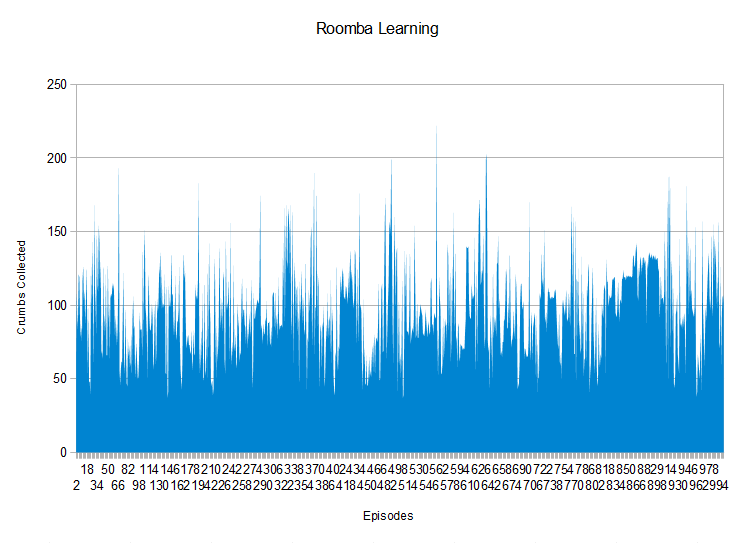
\includegraphics[height=7cm]{figs/roomba_learning_1000gen.png}
	\end{center}
}

%\frame{
%    \frametitle{Conclusions}
%	\begin{itemize}
%	\item The formal conclusion has not been decided yet.
%	\end{itemize}
%}

%\frame{
%    \frametitle{Future Work}
%}

\section{Discussion}
\frame{
    \frametitle{Discussion Time}
    \begin{itemize}
        \item Any questions or suggestions?  \\
            \begin{figure}
                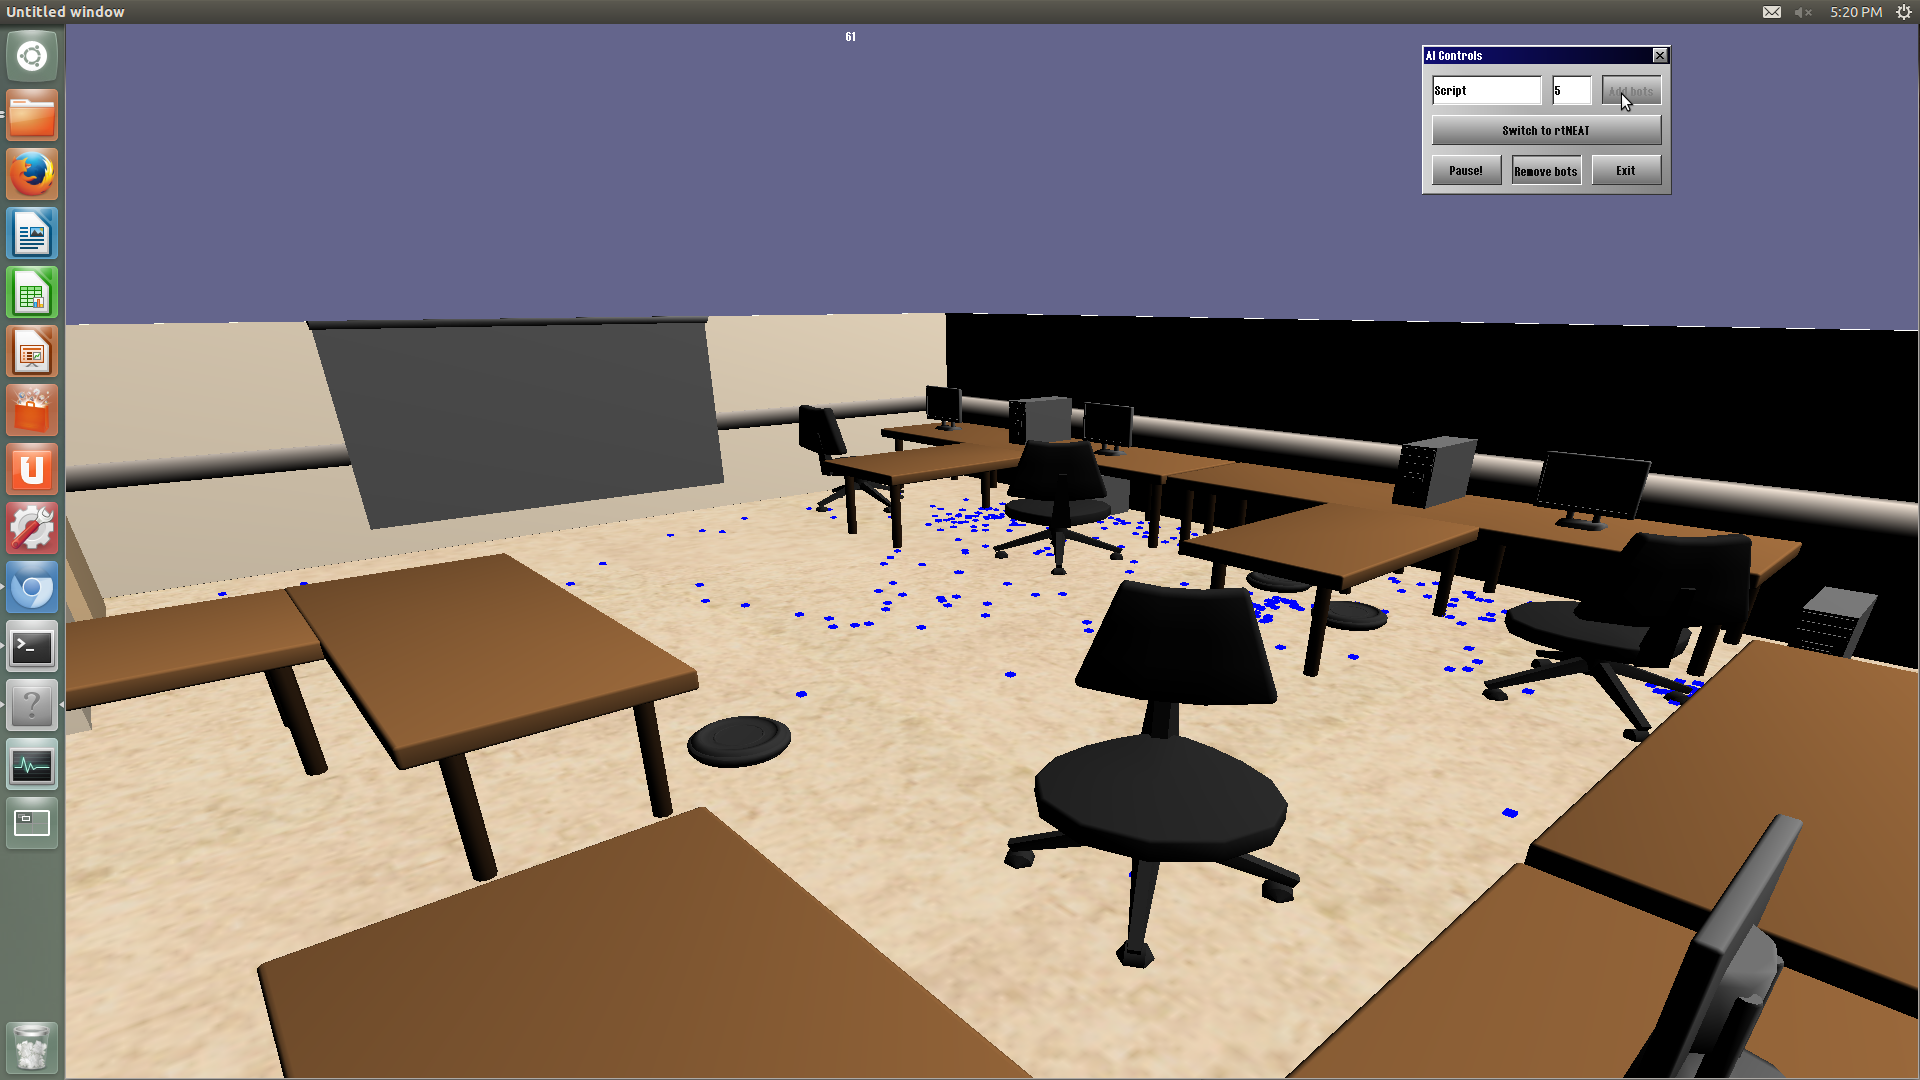
\includegraphics[width=4.5cm]{./figs/roomba1.png}
                %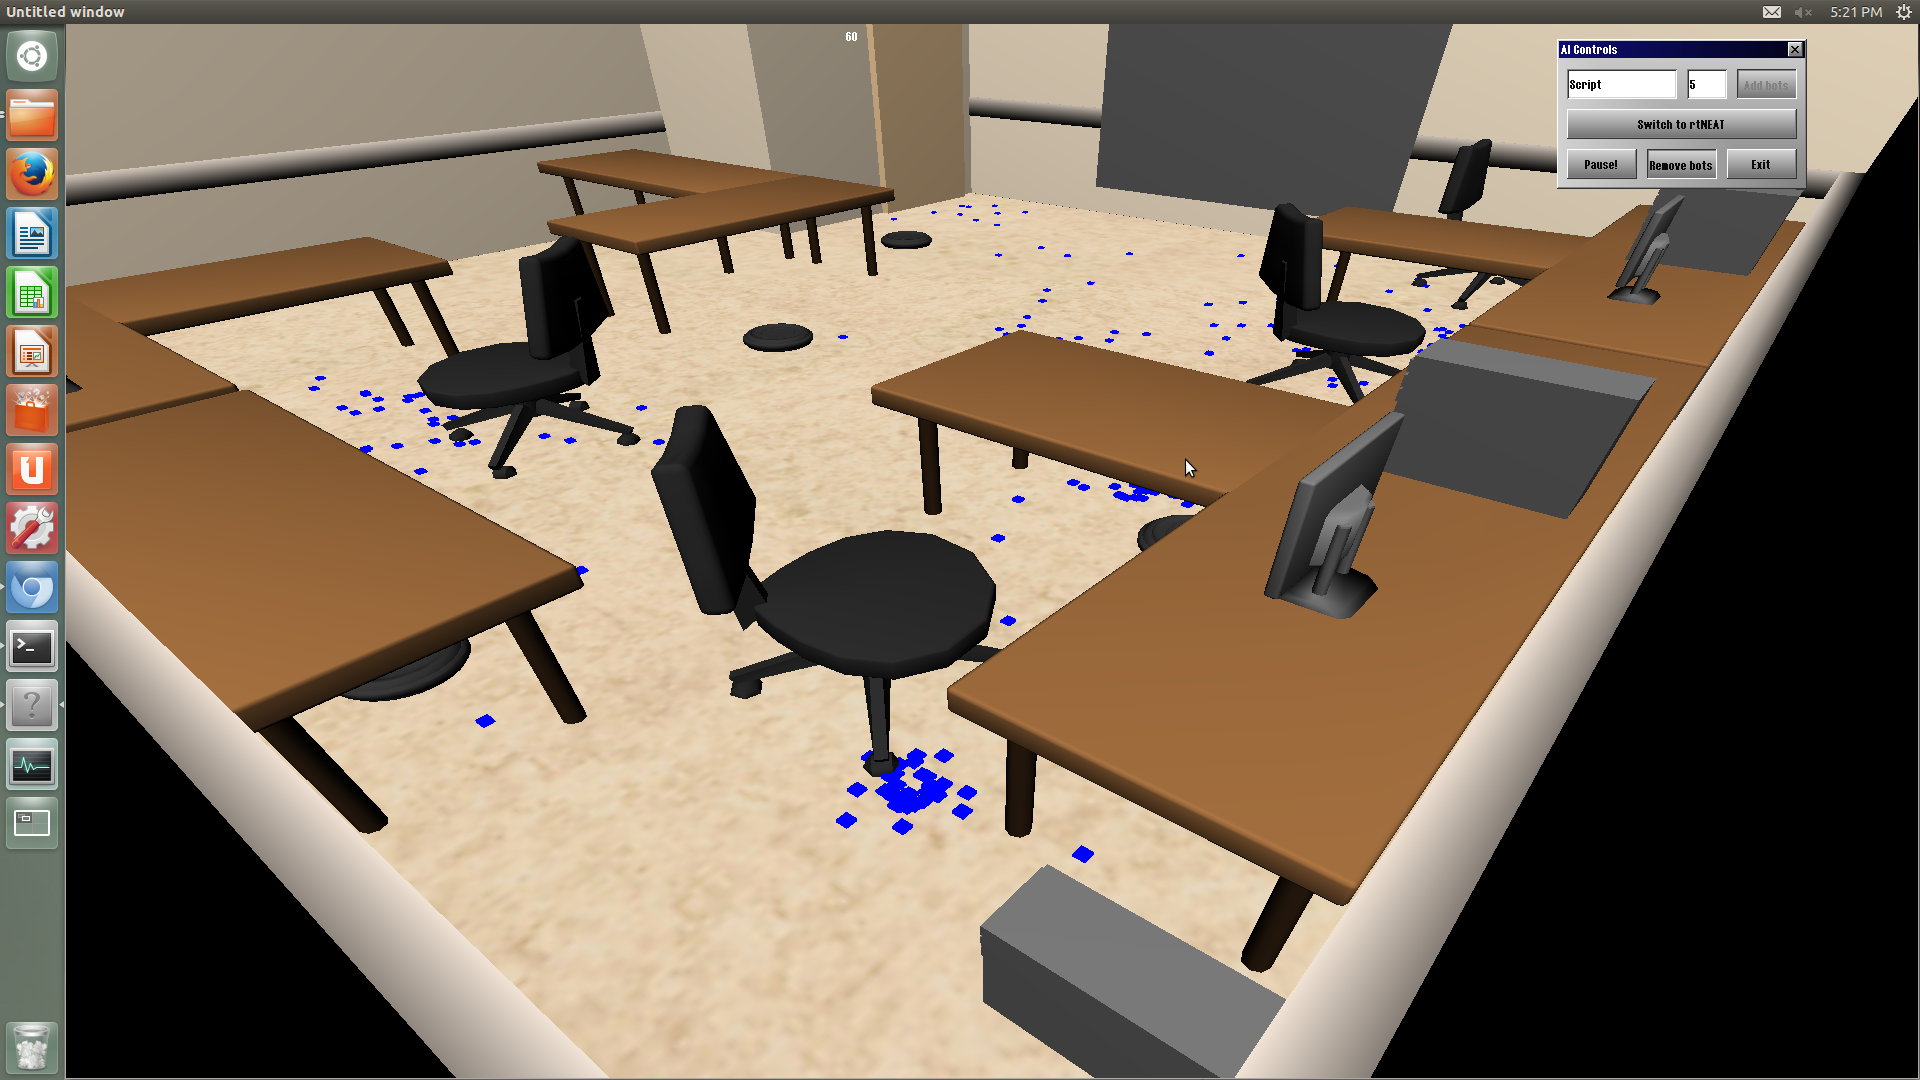
\includegraphics[width=5cm]{./figs/roomba2.png}
                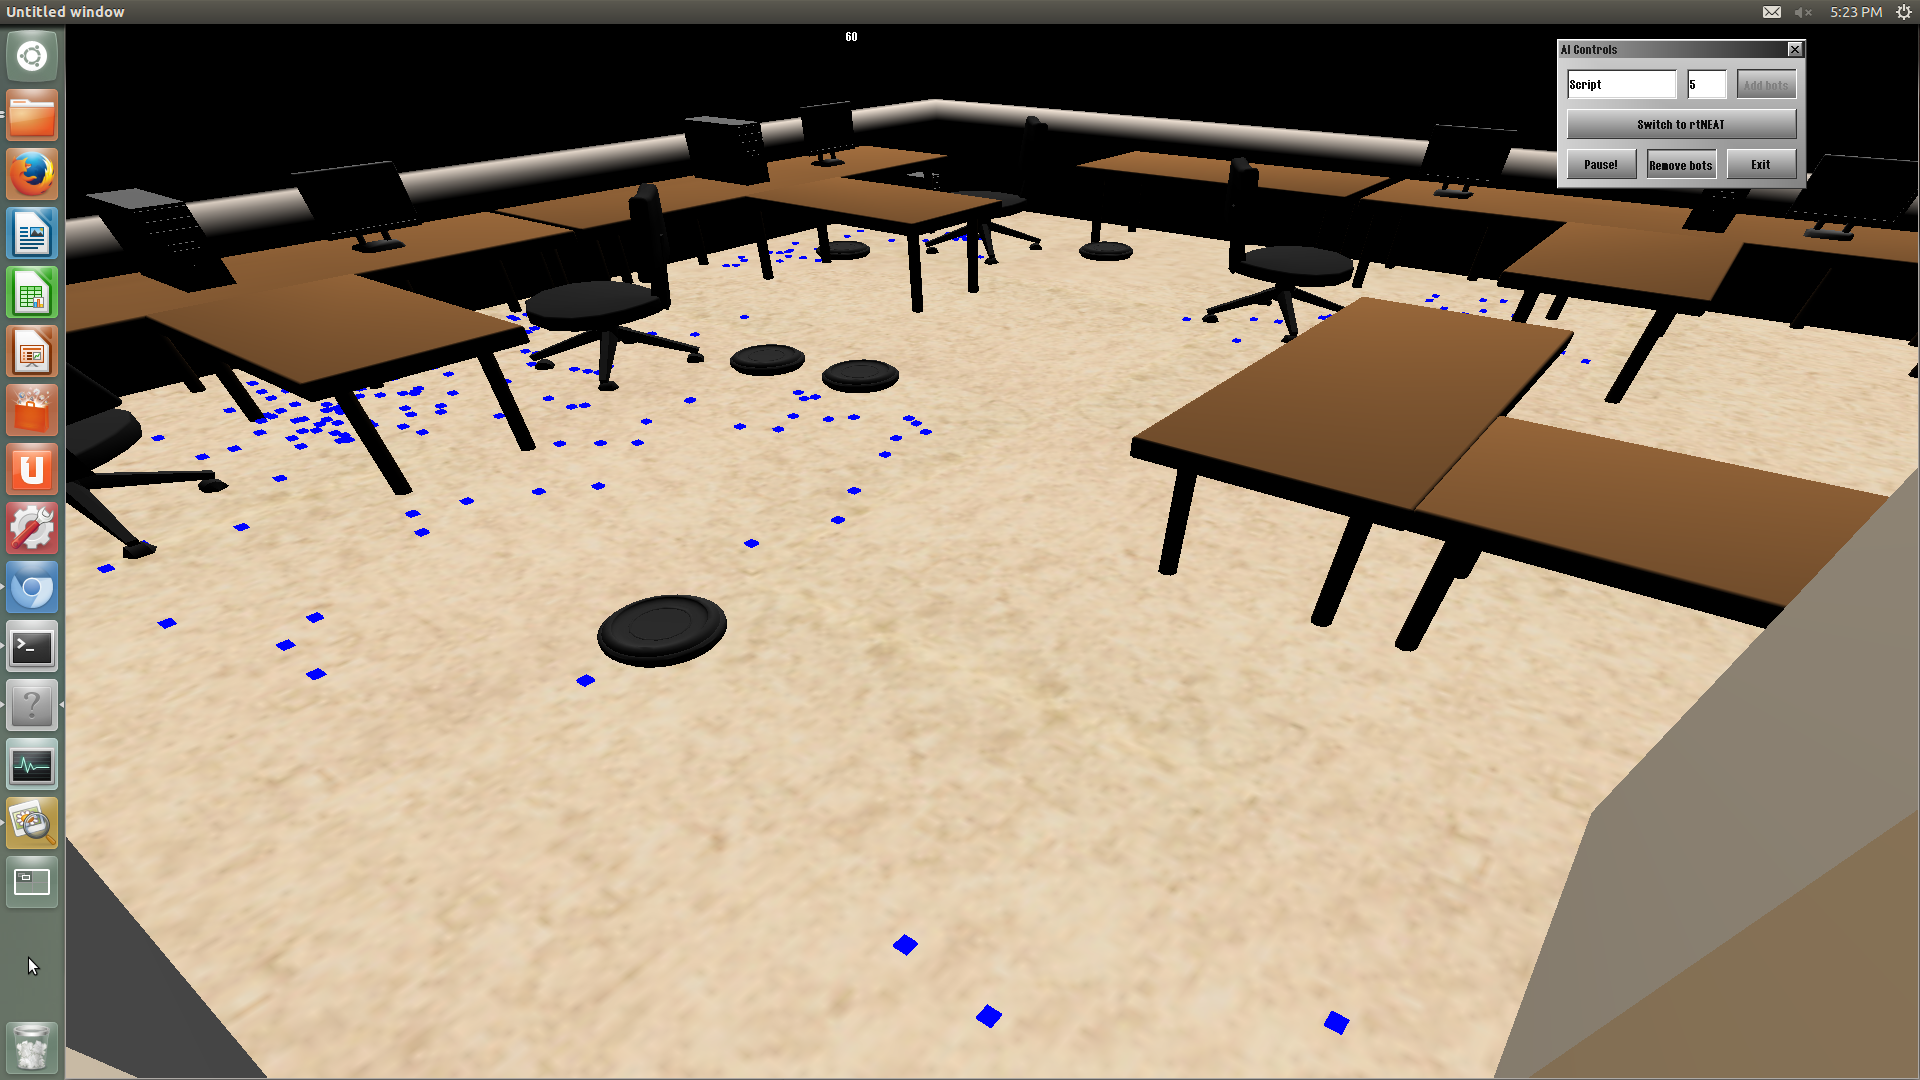
\includegraphics[width=4.5cm]{./figs/roomba3.png}
            \end{figure}
        \item Or email us at 
            \begin{itemize}
                \item jimmylin at utexas dot edu
                \item chevron8 at gmail dot com
            \end{itemize}
    \end{itemize}
}

%%%%%%%%%%%%%%%%%%%%%%%%%%%%%%%%%%%%%%%%%%%%%%%%%%%%%%%%%%%%%%%%%%%%%%%%
%%% REFERENCES
%%%%%%%%%%%%%%%%%%%%%%%%%%%%%%%%%%%%%%%%%%%%%%%%%%%%%%%%%%%%%%%%%%%%%%%%
%\appendix
%\section{Appendix}
%\frame[allowframebreaks]{
%    \frametitle{References}
%    \begin{thebibliography}{9}
%    	\bibitem{bryant03} Bobby D. Bryant and Risto Miikkulainen (2003). Neuroevolution for Adaptive Teams. {\it Proceedings of the 2003 Congress on Evolutionary Computation} 1:2194-2201. 
%    
%        \bibitem{tan1993multi} Tan, Ming. "Multi-agent reinforcement learning:
%        Independent vs. cooperative agents." {\it Proceedings of the Tenth
%            International Conference on Machine Learning}. Vol. 337. 1993.
%        
%        \bibitem{rawar} Rawal, A.; Rajagopalan, P.; Miikkulainen, R., "Constructing competitive and cooperative agent behavior using coevolution," {\it Computational Intelligence and Games (CIG), 2010 IEEE Symposium on}, vol., no., pp.107,114, 18-21 Aug. 2010
%        
%        \bibitem{rajagopalan11} Rajagopalan, P.; Rawal, A.; Miikkulainen, R.; Wiseman, M.A.; Holekamp, K.E., "The role of reward structure, coordination mechanism and net return in the evolution of cooperation," {\it Computational Intelligence and Games (CIG), 2011 IEEE Conference on}, vol., no., pp.258,265, Aug. 31 2011-Sept. 3 2011
%        
%    	\bibitem{risto12} Risto Miikkulainen and Eliana Feasley and Leif Johnson and Igor Karpov and Padmini Rajagopalan and Aditya Rawal and Wesley Tansey (2012). {\it Multiagent Learning through Neuroevolution. Advances in Computational Intelligence} LNCS 7311:24-46.     
%        
%        \bibitem{yang02} Yanli Yang; Polycarpou, M.M.; Minai, A.A., "Opportunistically cooperative neural learning in mobile agents," {\it Neural Networks, 2002. IJCNN '02. Proceedings of the 2002 International Joint Conference on}, vol.3, no., pp.2638,2643, 2002
%        
%        \bibitem{yong09} Yong, C.H.; Miikkulainen, R., "Coevolution of Role-Based Cooperation in Multiagent Systems," {\it Autonomous Mental Development, IEEE Transactions on}, vol.1, no.3, pp.170,186, Oct. 2009
%    \end{thebibliography}
%}

\frame{
    \frametitle{Acknowledgement}
    Thanks.
}
\end{document}
